\setcounter{page}{2}

\addchap{Цели работы}

Основной целью работы является изучение архитектуры гетерогенных вычислительных систем и технологии разработки ускорителей вычислений на базе ПЛИС фирмы Xilinx. В ходе лабораторной работы будут изучены основные сведения о платформе Xilinx Alveo U200,
разработано RTL (Register Transfer Language, язык регистровых передач) описание ускорителя вычислений по индивидуальному варианту, выполнена генерацию ядра ускорителя, выполнены синтез и сборка бинарного модуля ускорителя, разработаны и отлажены тестирующее программное обеспечение на серверной хост-платформе, проведены
тесты работы ускорителя вычислений. 

\textbf{В данной работе будет выполнен 12 вариант.}

\chapter{Функциональная схема}

На рис. 1.1 представлена функциональная схема разрабатываемой аппаратной системы. Дальнейшая работа будет выполняться по ней.

\captionsetup{singlelinecheck = false, justification=centering}
\begin{figure}[H]
	\begin{center}
		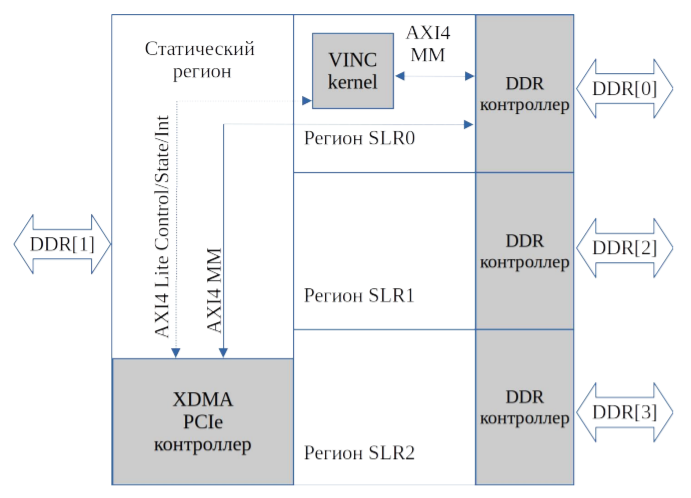
\includegraphics[scale=0.8]{assets/scheme.png}
	\end{center}
	\caption{Функциональная схема разрабатываемой аппаратной системы}
\end{figure}

\chapter{Изучение работы шины AXI}

На рис. 2.1 - 2.3 представлены транзакции чтения данных вектора на шине AXI4 MM из DDR памяти, записи результата инкремента данных на шине и инкремент данных в модуле rtl\_kernel\_wizard\_0\_example\_adder.v исходной симуляции.

\begin{figure}[H]
	\begin{center}
		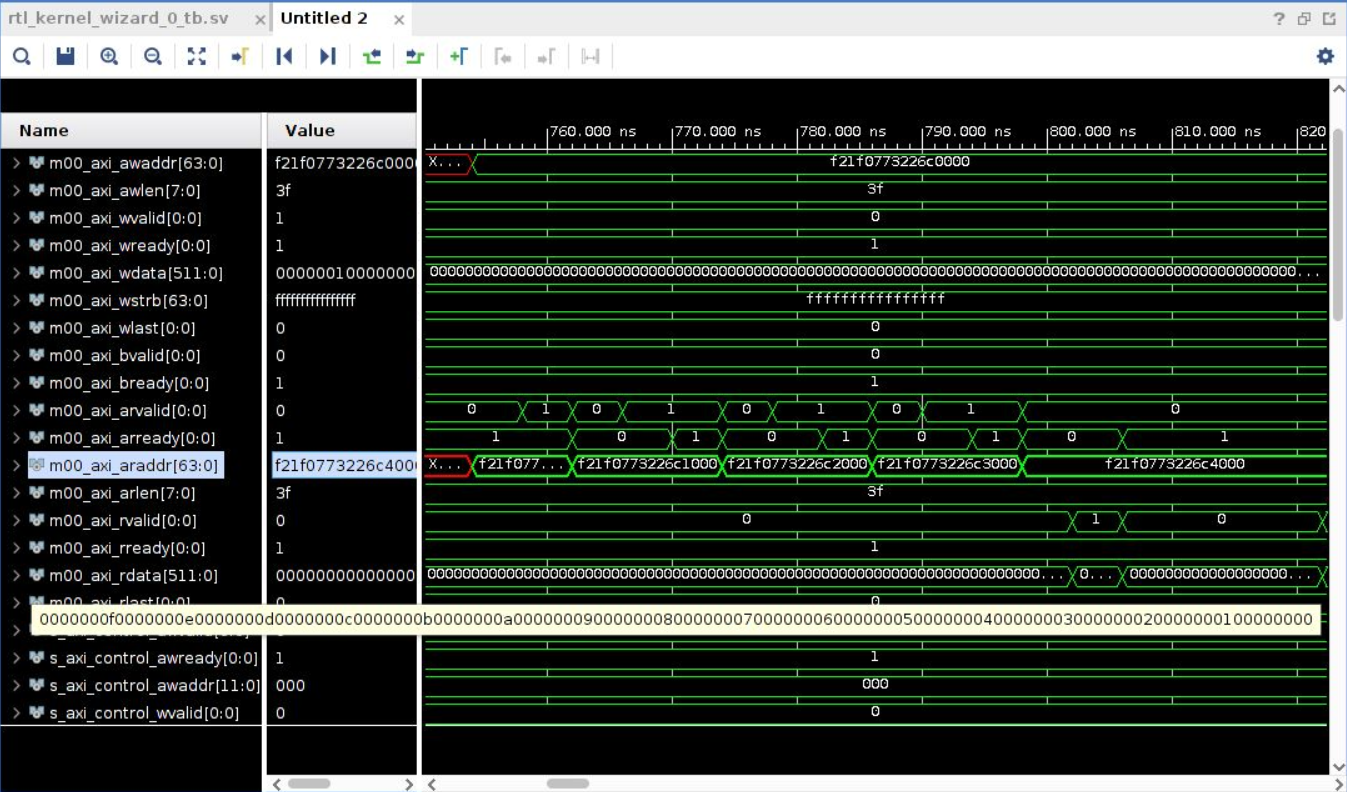
\includegraphics[scale=0.5]{assets/read_def.png}
	\end{center}
	\caption{Транзакции чтения данных вектора}
\end{figure}

\begin{figure}[H]
	\begin{center}
		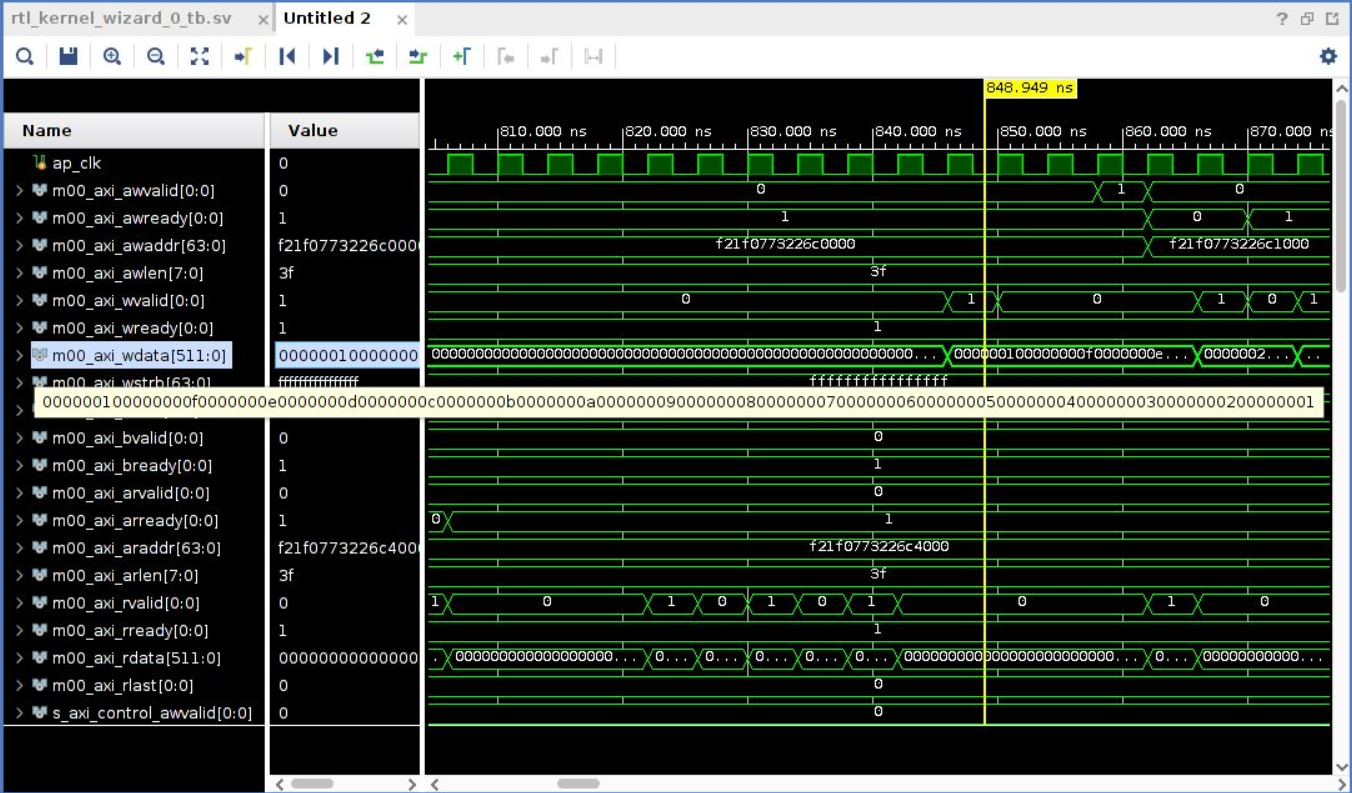
\includegraphics[scale=0.5]{assets/write_def.png}
	\end{center}
	\caption{Транзакции записи результата инкремента данных}
\end{figure}

Исходя из данных диаграмм, можно заметить, что считанные данные были инкрементированы корректно.

\begin{figure}[H]
	\begin{center}
		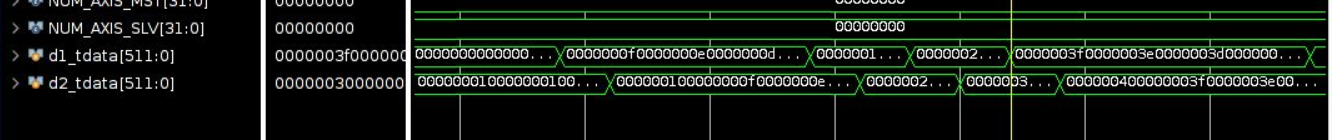
\includegraphics[scale=0.5]{assets/inc_def.png}
	\end{center}
	\caption{Инкремент данных}
\end{figure}

Теперь изменим rtl\_kernel\_wizard\_0\_example\_adder.v в соответствии с индивидуальным заданием (вариант 12), чтобы ускоритель выполнял требуемую функцию:
\begin{equation}
	R[i] = (A[i] \& 0xf0f0f0f0f0f0f0f0f0f0) + 10
\end{equation}

Код функции указан в листинге ниже.

\begin{lstlisting}[label=code, caption=Код инкремента данных]
// Adder function
always @(posedge s_axis_aclk) begin
	for (i = 0; i < LP_NUM_LOOPS; i = i + 1) begin
		d2_tdata[i*C_ADDER_BIT_WIDTH+:C_ADDER_BIT_WIDTH] <=
		d1_tdata[C_ADDER_BIT_WIDTH*i+:C_ADDER_BIT_WIDTH] &
		'hf0f0f0f0f0 + 10;
	end
end
\end{lstlisting}
\captionsetup{singlelinecheck = false, justification=centering}

На рис. 2.5 - 2.7 представлены представлены транзакции чтения данных вектора, записи результата инкремента данных и инкремент данных в rtl\_kernel\_wizard\_0\_example\_adder.v после изменения данного файла.

Также пришлось исправить модуль проверки в rtl\_kernel\_wizard\_0\_tb.sv, чтобы не возникало ошибок при проверке (рис. 2.4).

\begin{figure}[H]
	\begin{center}
		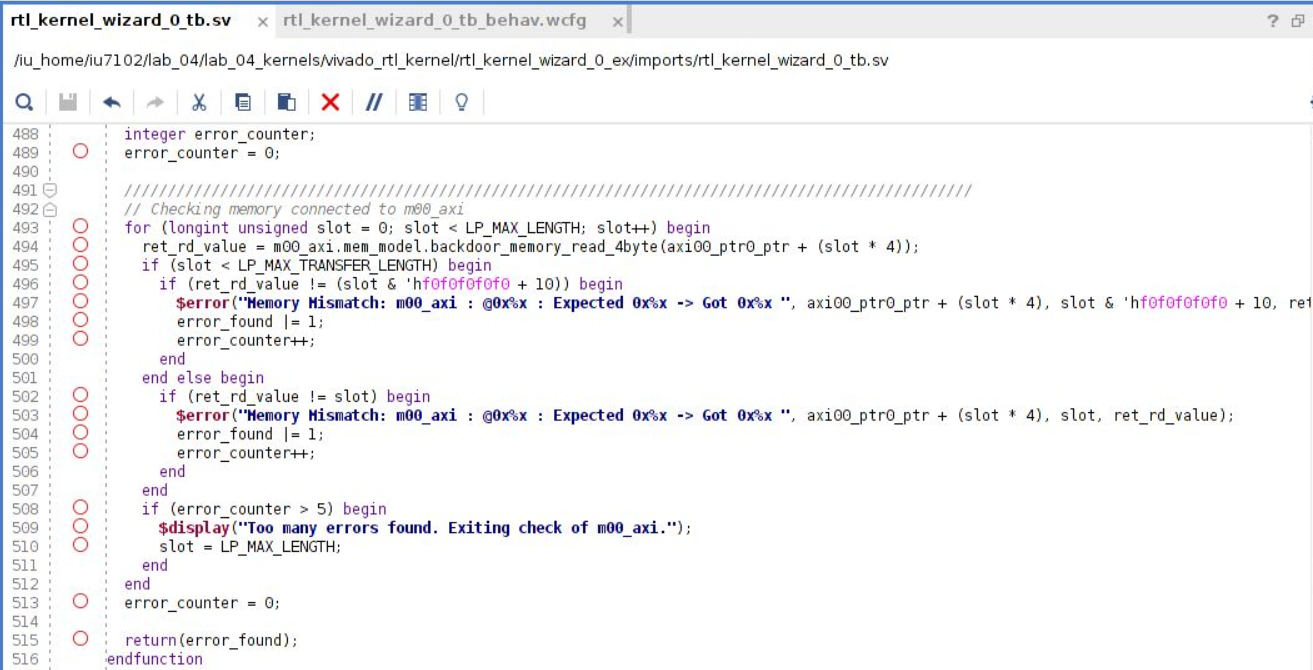
\includegraphics[scale=0.5]{assets/tb_fixed.png}
	\end{center}
	\caption{Код проверки в модуле rtl\_kernel\_wizard\_0\_tb.sv}
\end{figure}

\begin{figure}[H]
	\begin{center}
		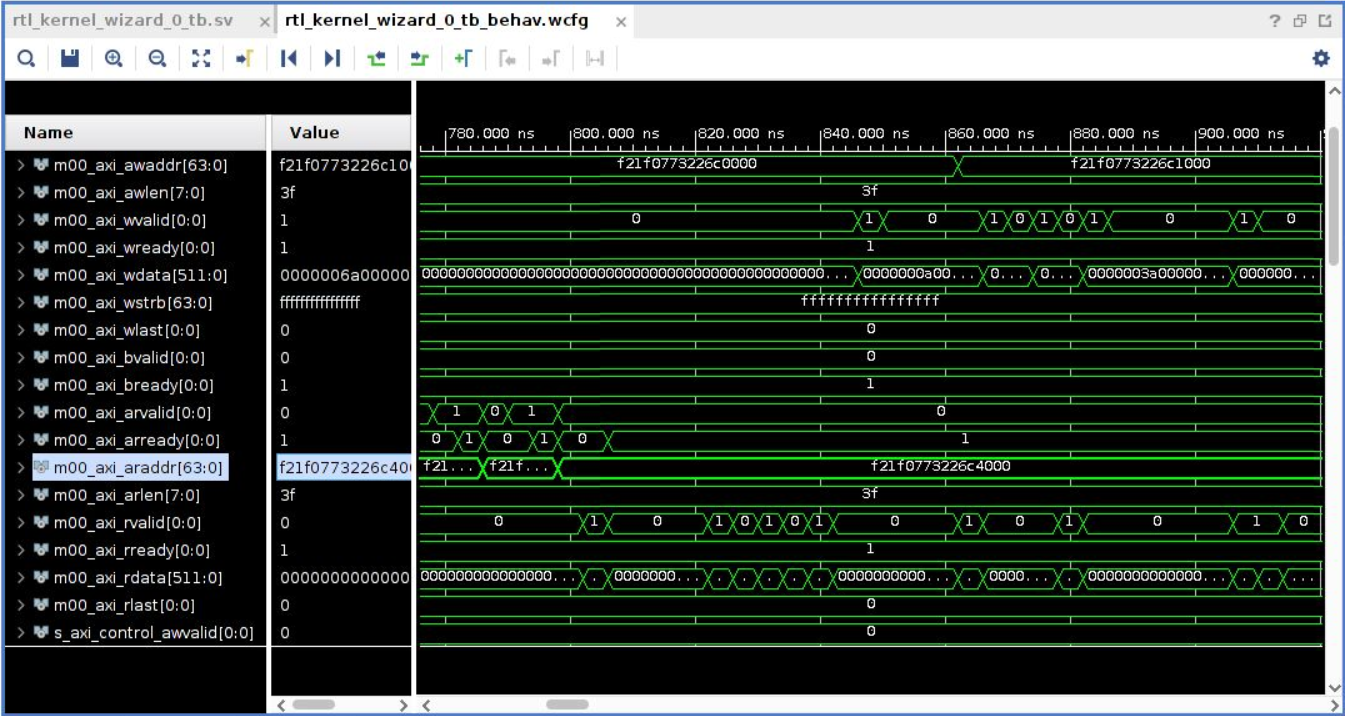
\includegraphics[scale=0.5]{assets/read.png}
	\end{center}
	\caption{Транзакции чтения данных вектора}
\end{figure}

\begin{figure}[H]
	\begin{center}
		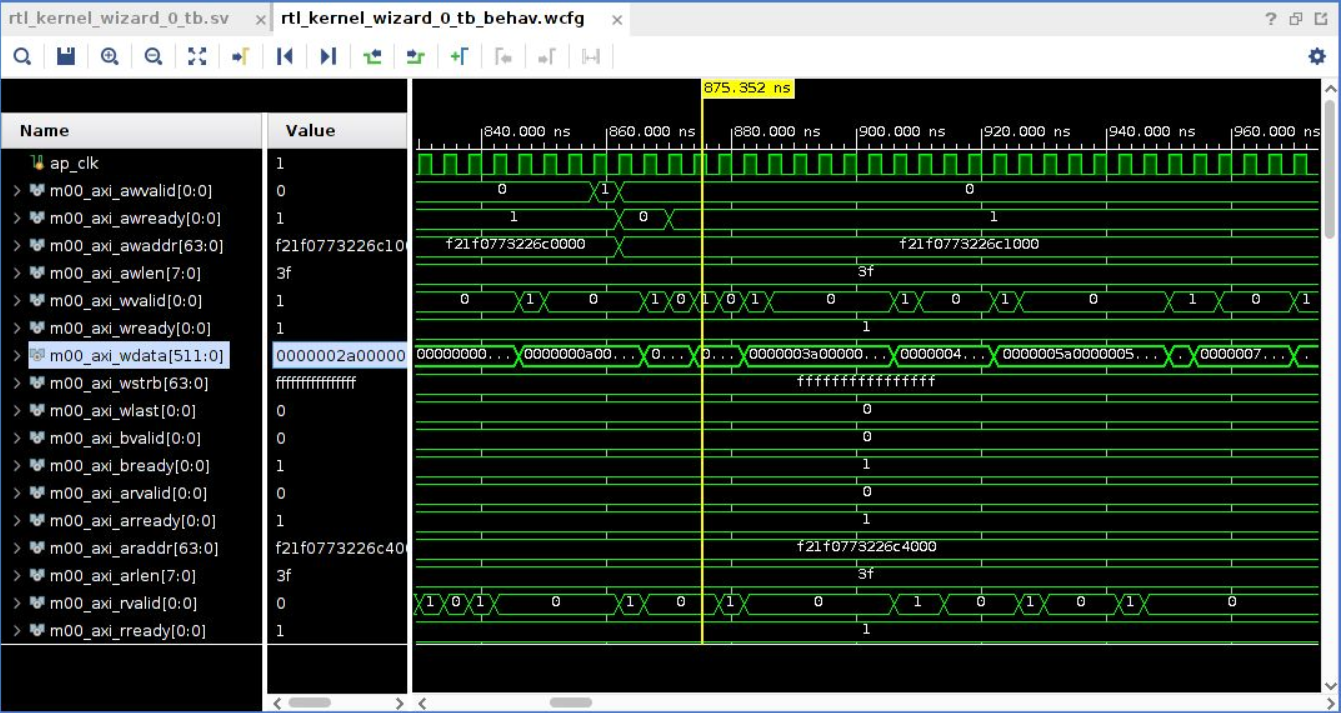
\includegraphics[scale=0.5]{assets/write.png}
	\end{center}
	\caption{Транзакции записи результата инкремента данных}
\end{figure}

\begin{figure}[H]
	\begin{center}
		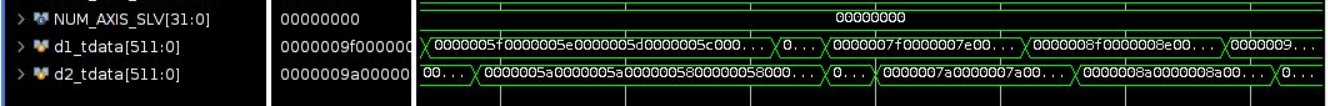
\includegraphics[scale=0.5]{assets/inc.png}
	\end{center}
	\caption{Инкремент данных}
\end{figure}

\chapter{Сборка проекта}

Был создан конфигурационный файл, листинг которого представлен ниже.

\begin{lstlisting}[label=code, caption=Листинг конфигурационного файла rtl\_kernel\_wizard\_0.cfg]
[connectivity]
nk=rtl_kernel_wizard_0:1:vinc0
slr=vinc0:SLR2
sp=vinc0.m00_axi:DDR[3]

[vivado]
prop=run.impl_1.STEPS.OPT_DESIGN.ARGS.DIRECTIVE=Explore
prop=run.impl_1.STEPS.PLACE_DESIGN.ARGS.DIRECTIVE=Explore
prop=run.impl_1.STEPS.PHYS_OPT_DESIGN.IS_ENABLED=true
prop=run.impl_1.STEPS.PHYS_OPT_DESIGN.ARGS.DIRECTIVE=AggressiveExplore
prop=run.impl_1.STEPS.ROUTE_DESIGN.ARGS.DIRECTIVE=Explore
\end{lstlisting}

В приложении A представлен листинг файла v++\_vinc.log, в приложении Б - vinc.xclbin.info.

\chapter{Тестирование}

Для тестирования используется программа, код которой представлен в файле host\_example.cpp (полный листинг в приложении В). Ниже представлена измененная часть, в соответствии с вариантом.
\begin{lstlisting}[label=code, caption=Модифицированный модуль host\_example.cpp]
for (cl_uint i = 0; i < number_of_words; i++) {
        if ((h_data[i] & 0xf0f0f0f0f0 + 10) != h_axi00_ptr0_output[i]) {
            printf("ERROR in rtl_kernel_wizard_0::m00_axi - array index
             %d (host addr 0x%03x) - input=%d (0x%x), output=%d (0x%x)\n",
             i, i*4, h_data[i], h_data[i], h_axi00_ptr0_output[i],
             h_axi00_ptr0_output[i]);
            check_status = 1;
		}
\end{lstlisting}

На рис. 4.1 и 4.2 представлено тестирование проекта.

\begin{figure}[H]
	\begin{center}
		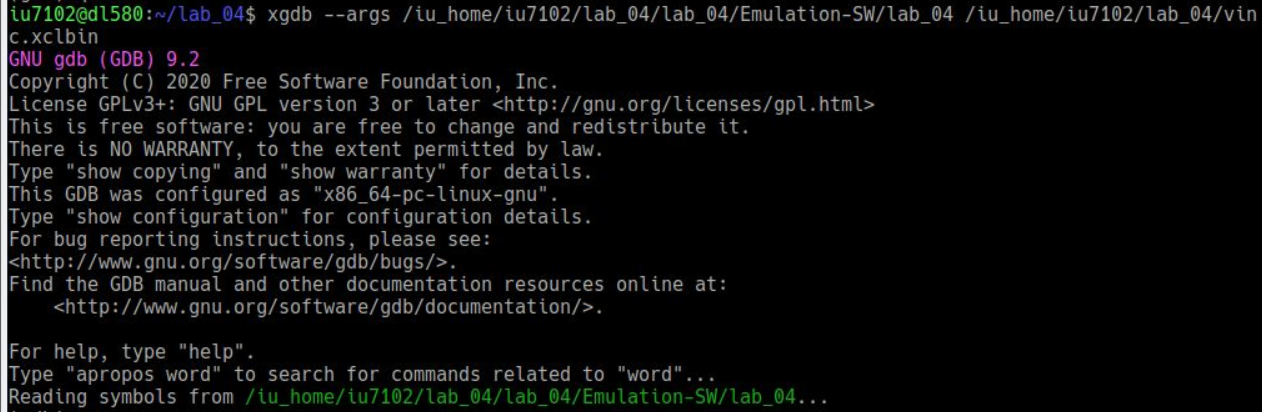
\includegraphics[scale=0.6]{assets/gdb_start.png}
	\end{center}
	\caption{Тестирование}
\end{figure}

\begin{figure}[H]
	\begin{center}
		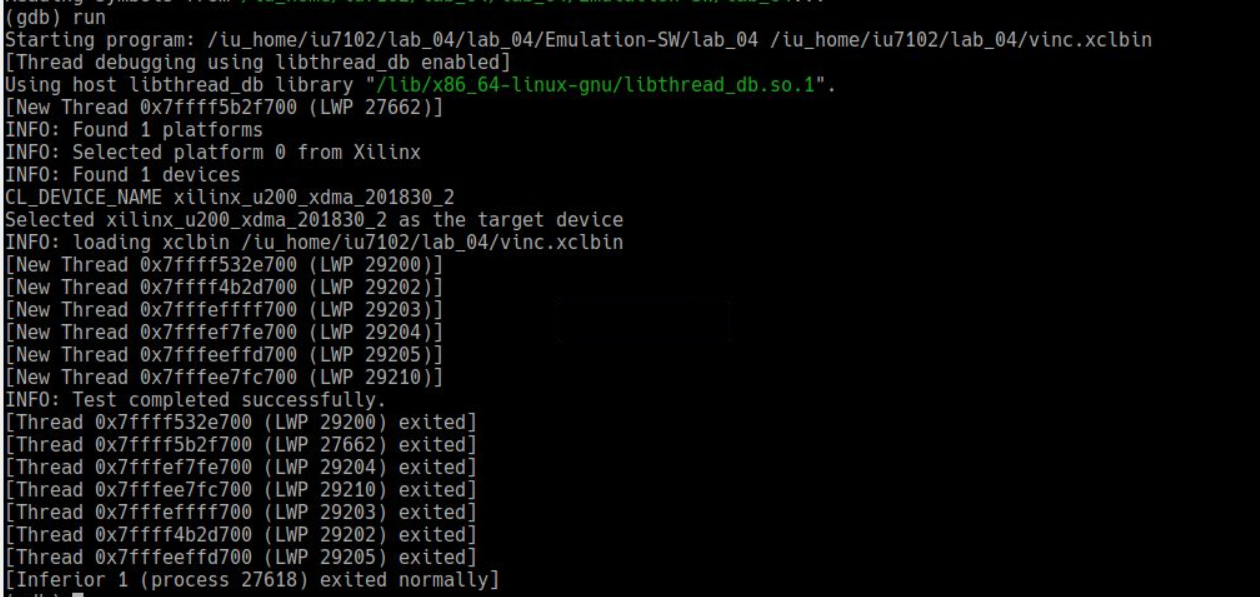
\includegraphics[scale=0.6]{assets/gdb_finish.png}
	\end{center}
	\caption{Тестирование (часть 2)}
\end{figure}

Все тесты пройдены успешно, а значит программа на ускорителе работает корректно.

\addchap{Вывод}

В ходе лабораторной работы были изучены основные сведения о платформе Xilinx Alveo U200, разработано RTL описание ускорителя по варианту, выполнена генерацию ядра ускорителя, выполнены синтез и сборка бинарного модуля ускорителя, разработаны и отлажены тестирующее программное обеспечение на серверной хост-платформе, проведены
тесты работы ускорителя вычислений. Поставленные цели были достигнуты.

\addchap{Приложение А}
\begin{lstlisting}[label=code, basicstyle=\tiny, caption=Листинг файла v++\_vinc.log]
INFO: [v++ 60-1306] Additional information associated with this v++ link can be found at:
	Reports: /iu_home/iu7102/lab_04/_x/reports/link
	Log files: /iu_home/iu7102/lab_04/_x/logs/link
INFO: [v++ 60-1548] Creating build summary session with primary output /iu_home/iu7102/lab_04/vinc.xclbin.link_summary, at Thu Jan  6 00:25:36 2022
INFO: [v++ 60-1316] Initiating connection to rulecheck server, at Thu Jan  6 00:25:36 2022
INFO: [v++ 60-1315] Creating rulecheck session with output '/iu_home/iu7102/lab_04/_x/reports/link/v++_link_vinc_guidance.html', at Thu Jan  6 00:25:55 2022
INFO: [v++ 60-895]   Target platform: /opt/xilinx/platforms/xilinx_u200_xdma_201830_2/xilinx_u200_xdma_201830_2.xpfm
INFO: [v++ 60-1578]   This platform contains Device Support Archive '/opt/xilinx/platforms/xilinx_u200_xdma_201830_2/hw/xilinx_u200_xdma_201830_2.dsa'
INFO: [v++ 74-74] Compiler Version string: 2020.2
INFO: [v++ 60-1302] Platform 'xilinx_u200_xdma_201830_2.xpfm' has been explicitly enabled for this release.
INFO: [v++ 60-629] Linking for hardware target
INFO: [v++ 60-423]   Target device: xilinx_u200_xdma_201830_2
INFO: [v++ 60-1332] Run 'run_link' status: Not started
INFO: [v++ 60-1443] [00:26:56] Run run_link: Step system_link: Started
INFO: [v++ 60-1453] Command Line: system_link --xo /iu_home/iu7102/lab_04/lab_04_kernels/vivado_rtl_kernel/rtl_kernel_wizard_0_ex/exports/rtl_kernel_wizard_0.xo --config /iu_home/iu7102/lab_04/_x/link/int/syslinkConfig.ini --xpfm /opt/xilinx/platforms/xilinx_u200_xdma_201830_2/xilinx_u200_xdma_201830_2.xpfm --target hw --output_dir /iu_home/iu7102/lab_04/_x/link/int --temp_dir /iu_home/iu7102/lab_04/_x/link/sys_link
INFO: [v++ 60-1454] Run Directory: /iu_home/iu7102/lab_04/_x/link/run_link
INFO: [SYSTEM_LINK 60-1316] Initiating connection to rulecheck server, at Thu Jan  6 00:27:11 2022
INFO: [SYSTEM_LINK 82-70] Extracting xo v3 file /iu_home/iu7102/lab_04/lab_04_kernels/vivado_rtl_kernel/rtl_kernel_wizard_0_ex/exports/rtl_kernel_wizard_0.xo
INFO: [SYSTEM_LINK 82-53] Creating IP database /iu_home/iu7102/lab_04/_x/link/sys_link/_sysl/.cdb/xd_ip_db.xml
INFO: [SYSTEM_LINK 82-38] [00:27:14] build_xd_ip_db started: /data/Xilinx/Vitis/2020.2/bin/build_xd_ip_db -ip_search 0  -sds-pf /iu_home/iu7102/lab_04/_x/link/sys_link/xilinx_u200_xdma_201830_2.hpfm -clkid 0 -ip /iu_home/iu7102/lab_04/_x/link/sys_link/iprepo/mycompany_com_kernel_rtl_kernel_wizard_0_1_0,rtl_kernel_wizard_0 -o /iu_home/iu7102/lab_04/_x/link/sys_link/_sysl/.cdb/xd_ip_db.xml
INFO: [SYSTEM_LINK 82-37] [00:27:49] build_xd_ip_db finished successfully
Time (s): cpu = 00:00:36 ; elapsed = 00:00:36 . Memory (MB): peak = 1557.898 ; gain = 0.000 ; free physical = 46268 ; free virtual = 282427
INFO: [SYSTEM_LINK 82-51] Create system connectivity graph
INFO: [SYSTEM_LINK 82-102] Applying explicit connections to the system connectivity graph: /iu_home/iu7102/lab_04/_x/link/sys_link/cfgraph/cfgen_cfgraph.xml
INFO: [SYSTEM_LINK 82-38] [00:27:50] cfgen started: /data/Xilinx/Vitis/2020.2/bin/cfgen  -nk rtl_kernel_wizard_0:1:vinc0 -slr vinc0:SLR2 -sp vinc0.m00_axi:DDR[3] -dmclkid 0 -r /iu_home/iu7102/lab_04/_x/link/sys_link/_sysl/.cdb/xd_ip_db.xml -o /iu_home/iu7102/lab_04/_x/link/sys_link/cfgraph/cfgen_cfgraph.xml
INFO: [CFGEN 83-0] Kernel Specs: 
INFO: [CFGEN 83-0]   kernel: rtl_kernel_wizard_0, num: 1  {vinc0}
INFO: [CFGEN 83-0] Port Specs: 
INFO: [CFGEN 83-0]   kernel: vinc0, k_port: m00_axi, sptag: DDR[3]
INFO: [CFGEN 83-0] SLR Specs: 
INFO: [CFGEN 83-0]   instance: vinc0, SLR: SLR2
INFO: [CFGEN 83-2228] Creating mapping for argument vinc0.axi00_ptr0 to DDR[3] for directive vinc0.m00_axi:DDR[3]
INFO: [SYSTEM_LINK 82-37] [00:28:16] cfgen finished successfully
Time (s): cpu = 00:00:26 ; elapsed = 00:00:27 . Memory (MB): peak = 1557.898 ; gain = 0.000 ; free physical = 45902 ; free virtual = 282054
INFO: [SYSTEM_LINK 82-52] Create top-level block diagram
INFO: [SYSTEM_LINK 82-38] [00:28:16] cf2bd started: /data/Xilinx/Vitis/2020.2/bin/cf2bd  --linux --trace_buffer 1024 --input_file /iu_home/iu7102/lab_04/_x/link/sys_link/cfgraph/cfgen_cfgraph.xml --ip_db /iu_home/iu7102/lab_04/_x/link/sys_link/_sysl/.cdb/xd_ip_db.xml --cf_name dr --working_dir /iu_home/iu7102/lab_04/_x/link/sys_link/_sysl/.xsd --temp_dir /iu_home/iu7102/lab_04/_x/link/sys_link --output_dir /iu_home/iu7102/lab_04/_x/link/int --target_bd pfm_dynamic.bd
INFO: [CF2BD 82-31] Launching cf2xd: cf2xd -linux -trace-buffer 1024 -i /iu_home/iu7102/lab_04/_x/link/sys_link/cfgraph/cfgen_cfgraph.xml -r /iu_home/iu7102/lab_04/_x/link/sys_link/_sysl/.cdb/xd_ip_db.xml -o dr.xml
INFO: [CF2BD 82-28] cf2xd finished successfully
INFO: [CF2BD 82-31] Launching cf_xsd: cf_xsd -disable-address-gen -bd pfm_dynamic.bd -dn dr -dp /iu_home/iu7102/lab_04/_x/link/sys_link/_sysl/.xsd
INFO: [CF2BD 82-28] cf_xsd finished successfully
INFO: [SYSTEM_LINK 82-37] [00:28:32] cf2bd finished successfully
Time (s): cpu = 00:00:13 ; elapsed = 00:00:16 . Memory (MB): peak = 1557.898 ; gain = 0.000 ; free physical = 45998 ; free virtual = 282142
INFO: [v++ 60-1441] [00:28:33] Run run_link: Step system_link: Completed
Time (s): cpu = 00:01:31 ; elapsed = 00:01:36 . Memory (MB): peak = 1585.129 ; gain = 0.000 ; free physical = 46083 ; free virtual = 282223
INFO: [v++ 60-1443] [00:28:33] Run run_link: Step cf2sw: Started
INFO: [v++ 60-1453] Command Line: cf2sw -sdsl /iu_home/iu7102/lab_04/_x/link/int/sdsl.dat -rtd /iu_home/iu7102/lab_04/_x/link/int/cf2sw.rtd -nofilter /iu_home/iu7102/lab_04/_x/link/int/cf2sw_full.rtd -xclbin /iu_home/iu7102/lab_04/_x/link/int/xclbin_orig.xml -o /iu_home/iu7102/lab_04/_x/link/int/xclbin_orig.1.xml
INFO: [v++ 60-1454] Run Directory: /iu_home/iu7102/lab_04/_x/link/run_link
INFO: [v++ 60-1441] [00:28:51] Run run_link: Step cf2sw: Completed
Time (s): cpu = 00:00:16 ; elapsed = 00:00:18 . Memory (MB): peak = 1585.129 ; gain = 0.000 ; free physical = 46018 ; free virtual = 282162
INFO: [v++ 60-1443] [00:28:51] Run run_link: Step rtd2_system_diagram: Started
INFO: [v++ 60-1453] Command Line: rtd2SystemDiagram
INFO: [v++ 60-1454] Run Directory: /iu_home/iu7102/lab_04/_x/link/run_link
INFO: [v++ 60-1441] [00:29:02] Run run_link: Step rtd2_system_diagram: Completed
Time (s): cpu = 00:00:00.02 ; elapsed = 00:00:12 . Memory (MB): peak = 1585.129 ; gain = 0.000 ; free physical = 45910 ; free virtual = 282058
INFO: [v++ 60-1443] [00:29:02] Run run_link: Step vpl: Started
INFO: [v++ 60-1453] Command Line: vpl -t hw -f xilinx_u200_xdma_201830_2 --remote_ip_cache /iu_home/iu7102/lab_04/.ipcache --output_dir /iu_home/iu7102/lab_04/_x/link/int --log_dir /iu_home/iu7102/lab_04/_x/logs/link --report_dir /iu_home/iu7102/lab_04/_x/reports/link --config /iu_home/iu7102/lab_04/_x/link/int/vplConfig.ini -k /iu_home/iu7102/lab_04/_x/link/int/kernel_info.dat --webtalk_flag Vitis --temp_dir /iu_home/iu7102/lab_04/_x/link --no-info --iprepo /iu_home/iu7102/lab_04/_x/link/int/xo/ip_repo/mycompany_com_kernel_rtl_kernel_wizard_0_1_0 --messageDb /iu_home/iu7102/lab_04/_x/link/run_link/vpl.pb /iu_home/iu7102/lab_04/_x/link/int/dr.bd.tcl
INFO: [v++ 60-1454] Run Directory: /iu_home/iu7102/lab_04/_x/link/run_link

****** vpl v2020.2 (64-bit)
  **** SW Build (by xbuild) on 2020-11-18-05:13:29
    ** Copyright 1986-2020 Xilinx, Inc. All Rights Reserved.

INFO: [VPL 60-839] Read in kernel information from file '/iu_home/iu7102/lab_04/_x/link/int/kernel_info.dat'.
INFO: [VPL 74-74] Compiler Version string: 2020.2
INFO: [VPL 60-423]   Target device: xilinx_u200_xdma_201830_2
INFO: [VPL 60-1032] Extracting hardware platform to /iu_home/iu7102/lab_04/_x/link/vivado/vpl/.local/hw_platform
WARNING: /data/Xilinx/Vitis/2020.2/tps/lnx64/jre9.0.4 does not exist.
[00:35:58] Run vpl: Step create_project: RUNNING...
[00:35:52] Run vpl: Step create_project: Started
Creating Vivado project.
[00:36:27] Run vpl: Step create_project: Completed
[00:36:27] Run vpl: Step create_bd: Started
[00:38:08] Run vpl: Step create_bd: RUNNING...
[00:39:55] Run vpl: Step create_bd: RUNNING...
[00:41:34] Run vpl: Step create_bd: RUNNING...
[00:43:28] Run vpl: Step create_bd: RUNNING...
[00:45:17] Run vpl: Step create_bd: RUNNING...
[00:46:58] Run vpl: Step create_bd: RUNNING...
[00:48:24] Run vpl: Step create_bd: Completed
[00:48:24] Run vpl: Step update_bd: Started
[00:48:27] Run vpl: Step update_bd: Completed
[00:48:27] Run vpl: Step generate_target: Started
[00:50:03] Run vpl: Step generate_target: RUNNING...
[00:51:44] Run vpl: Step generate_target: RUNNING...
[00:53:14] Run vpl: Step generate_target: RUNNING...
[00:54:49] Run vpl: Step generate_target: RUNNING...
[00:56:16] Run vpl: Step generate_target: RUNNING...
[00:57:50] Run vpl: Step generate_target: RUNNING...
[00:59:18] Run vpl: Step generate_target: RUNNING...
[01:00:49] Run vpl: Step generate_target: RUNNING...
[01:01:14] Run vpl: Step generate_target: Completed
[01:01:14] Run vpl: Step config_hw_runs: Started
[01:02:51] Run vpl: Step config_hw_runs: Completed
[01:02:51] Run vpl: Step synth: Started
[01:05:21] Block-level synthesis in progress, 0 of 66 jobs complete, 8 jobs running.
[01:05:56] Block-level synthesis in progress, 0 of 66 jobs complete, 8 jobs running.
[01:06:33] Block-level synthesis in progress, 0 of 66 jobs complete, 8 jobs running.
[01:07:11] Block-level synthesis in progress, 0 of 66 jobs complete, 8 jobs running.
[01:07:49] Block-level synthesis in progress, 0 of 66 jobs complete, 8 jobs running.
[01:08:26] Block-level synthesis in progress, 0 of 66 jobs complete, 8 jobs running.
[01:09:04] Block-level synthesis in progress, 0 of 66 jobs complete, 8 jobs running.
[01:09:41] Block-level synthesis in progress, 0 of 66 jobs complete, 8 jobs running.
[01:10:20] Block-level synthesis in progress, 0 of 66 jobs complete, 8 jobs running.
[01:10:58] Block-level synthesis in progress, 0 of 66 jobs complete, 8 jobs running.
[01:11:37] Block-level synthesis in progress, 0 of 66 jobs complete, 8 jobs running.
[01:12:14] Block-level synthesis in progress, 1 of 66 jobs complete, 7 jobs running.
[01:12:55] Block-level synthesis in progress, 4 of 66 jobs complete, 4 jobs running.
[01:13:32] Block-level synthesis in progress, 6 of 66 jobs complete, 2 jobs running.
[01:14:13] Block-level synthesis in progress, 6 of 66 jobs complete, 5 jobs running.
[01:14:50] Block-level synthesis in progress, 6 of 66 jobs complete, 8 jobs running.
[01:15:28] Block-level synthesis in progress, 7 of 66 jobs complete, 7 jobs running.
[01:16:05] Block-level synthesis in progress, 8 of 66 jobs complete, 6 jobs running.
[01:16:49] Block-level synthesis in progress, 8 of 66 jobs complete, 6 jobs running.
[01:17:26] Block-level synthesis in progress, 8 of 66 jobs complete, 8 jobs running.
[01:18:06] Block-level synthesis in progress, 8 of 66 jobs complete, 8 jobs running.
[01:18:44] Block-level synthesis in progress, 8 of 66 jobs complete, 8 jobs running.
[01:19:25] Block-level synthesis in progress, 8 of 66 jobs complete, 8 jobs running.
[01:20:01] Block-level synthesis in progress, 8 of 66 jobs complete, 8 jobs running.
[01:20:41] Block-level synthesis in progress, 8 of 66 jobs complete, 8 jobs running.
[01:21:19] Block-level synthesis in progress, 8 of 66 jobs complete, 8 jobs running.
[01:21:58] Block-level synthesis in progress, 10 of 66 jobs complete, 6 jobs running.
[01:22:37] Block-level synthesis in progress, 11 of 66 jobs complete, 5 jobs running.
[01:23:17] Block-level synthesis in progress, 13 of 66 jobs complete, 5 jobs running.
[01:23:56] Block-level synthesis in progress, 13 of 66 jobs complete, 6 jobs running.
[01:24:35] Block-level synthesis in progress, 13 of 66 jobs complete, 8 jobs running.
[01:25:12] Block-level synthesis in progress, 15 of 66 jobs complete, 6 jobs running.
[01:25:54] Block-level synthesis in progress, 15 of 66 jobs complete, 6 jobs running.
[01:26:34] Block-level synthesis in progress, 16 of 66 jobs complete, 7 jobs running.
[01:27:12] Block-level synthesis in progress, 16 of 66 jobs complete, 7 jobs running.
[01:27:50] Block-level synthesis in progress, 16 of 66 jobs complete, 8 jobs running.
[01:28:29] Block-level synthesis in progress, 16 of 66 jobs complete, 8 jobs running.
[01:29:06] Block-level synthesis in progress, 16 of 66 jobs complete, 8 jobs running.
[01:29:45] Block-level synthesis in progress, 16 of 66 jobs complete, 8 jobs running.
[01:30:24] Block-level synthesis in progress, 16 of 66 jobs complete, 8 jobs running.
[01:31:05] Block-level synthesis in progress, 17 of 66 jobs complete, 7 jobs running.
[01:31:45] Block-level synthesis in progress, 18 of 66 jobs complete, 6 jobs running.
[01:32:29] Block-level synthesis in progress, 19 of 66 jobs complete, 7 jobs running.
[01:33:09] Block-level synthesis in progress, 19 of 66 jobs complete, 7 jobs running.
[01:33:49] Block-level synthesis in progress, 19 of 66 jobs complete, 8 jobs running.
[01:34:31] Block-level synthesis in progress, 19 of 66 jobs complete, 8 jobs running.
[01:35:12] Block-level synthesis in progress, 20 of 66 jobs complete, 7 jobs running.
[01:35:51] Block-level synthesis in progress, 21 of 66 jobs complete, 6 jobs running.
[01:36:34] Block-level synthesis in progress, 21 of 66 jobs complete, 7 jobs running.
[01:37:13] Block-level synthesis in progress, 21 of 66 jobs complete, 8 jobs running.
[01:37:53] Block-level synthesis in progress, 22 of 66 jobs complete, 7 jobs running.
[01:38:33] Block-level synthesis in progress, 23 of 66 jobs complete, 6 jobs running.
[01:39:15] Block-level synthesis in progress, 23 of 66 jobs complete, 7 jobs running.
[01:39:54] Block-level synthesis in progress, 23 of 66 jobs complete, 8 jobs running.
[01:40:36] Block-level synthesis in progress, 24 of 66 jobs complete, 7 jobs running.
[01:41:15] Block-level synthesis in progress, 25 of 66 jobs complete, 6 jobs running.
[01:42:00] Block-level synthesis in progress, 26 of 66 jobs complete, 5 jobs running.
[01:42:39] Block-level synthesis in progress, 26 of 66 jobs complete, 7 jobs running.
[01:43:18] Block-level synthesis in progress, 26 of 66 jobs complete, 7 jobs running.
[01:43:56] Block-level synthesis in progress, 26 of 66 jobs complete, 8 jobs running.
[01:44:39] Block-level synthesis in progress, 26 of 66 jobs complete, 8 jobs running.
[01:45:17] Block-level synthesis in progress, 26 of 66 jobs complete, 8 jobs running.
[01:46:01] Block-level synthesis in progress, 27 of 66 jobs complete, 7 jobs running.
[01:46:40] Block-level synthesis in progress, 27 of 66 jobs complete, 7 jobs running.
[01:47:22] Block-level synthesis in progress, 29 of 66 jobs complete, 6 jobs running.
[01:48:00] Block-level synthesis in progress, 29 of 66 jobs complete, 6 jobs running.
[01:48:43] Block-level synthesis in progress, 30 of 66 jobs complete, 7 jobs running.
[01:49:23] Block-level synthesis in progress, 31 of 66 jobs complete, 6 jobs running.
[01:50:03] Block-level synthesis in progress, 31 of 66 jobs complete, 7 jobs running.
[01:50:42] Block-level synthesis in progress, 32 of 66 jobs complete, 7 jobs running.
[01:51:21] Block-level synthesis in progress, 33 of 66 jobs complete, 6 jobs running.
[01:51:59] Block-level synthesis in progress, 34 of 66 jobs complete, 5 jobs running.
[01:52:40] Block-level synthesis in progress, 34 of 66 jobs complete, 7 jobs running.
[01:53:19] Block-level synthesis in progress, 36 of 66 jobs complete, 6 jobs running.
[01:53:58] Block-level synthesis in progress, 36 of 66 jobs complete, 6 jobs running.
[01:54:37] Block-level synthesis in progress, 36 of 66 jobs complete, 8 jobs running.
[01:55:16] Block-level synthesis in progress, 36 of 66 jobs complete, 8 jobs running.
[01:55:54] Block-level synthesis in progress, 37 of 66 jobs complete, 7 jobs running.
[01:56:37] Block-level synthesis in progress, 38 of 66 jobs complete, 6 jobs running.
[01:57:16] Block-level synthesis in progress, 38 of 66 jobs complete, 7 jobs running.
[01:57:55] Block-level synthesis in progress, 38 of 66 jobs complete, 8 jobs running.
[01:58:32] Block-level synthesis in progress, 39 of 66 jobs complete, 7 jobs running.
[01:59:11] Block-level synthesis in progress, 39 of 66 jobs complete, 7 jobs running.
[01:59:51] Block-level synthesis in progress, 39 of 66 jobs complete, 8 jobs running.
[02:00:32] Block-level synthesis in progress, 40 of 66 jobs complete, 7 jobs running.
[02:01:13] Block-level synthesis in progress, 40 of 66 jobs complete, 7 jobs running.
[02:01:52] Block-level synthesis in progress, 41 of 66 jobs complete, 7 jobs running.
[02:02:32] Block-level synthesis in progress, 42 of 66 jobs complete, 6 jobs running.
[02:03:12] Block-level synthesis in progress, 43 of 66 jobs complete, 6 jobs running.
[02:03:51] Block-level synthesis in progress, 43 of 66 jobs complete, 7 jobs running.
[02:04:29] Block-level synthesis in progress, 44 of 66 jobs complete, 7 jobs running.
[02:05:07] Block-level synthesis in progress, 45 of 66 jobs complete, 6 jobs running.
[02:05:47] Block-level synthesis in progress, 46 of 66 jobs complete, 6 jobs running.
[02:06:26] Block-level synthesis in progress, 47 of 66 jobs complete, 5 jobs running.
[02:07:07] Block-level synthesis in progress, 47 of 66 jobs complete, 7 jobs running.
[02:07:47] Block-level synthesis in progress, 48 of 66 jobs complete, 6 jobs running.
[02:08:27] Block-level synthesis in progress, 48 of 66 jobs complete, 7 jobs running.
[02:09:06] Block-level synthesis in progress, 48 of 66 jobs complete, 7 jobs running.
[02:09:46] Block-level synthesis in progress, 48 of 66 jobs complete, 8 jobs running.
[02:10:25] Block-level synthesis in progress, 49 of 66 jobs complete, 7 jobs running.
[02:11:06] Block-level synthesis in progress, 50 of 66 jobs complete, 6 jobs running.
[02:11:47] Block-level synthesis in progress, 51 of 66 jobs complete, 5 jobs running.
[02:12:30] Block-level synthesis in progress, 51 of 66 jobs complete, 7 jobs running.
[02:13:09] Block-level synthesis in progress, 54 of 66 jobs complete, 5 jobs running.
[02:13:49] Block-level synthesis in progress, 54 of 66 jobs complete, 5 jobs running.
[02:14:33] Block-level synthesis in progress, 54 of 66 jobs complete, 8 jobs running.
[02:15:10] Block-level synthesis in progress, 55 of 66 jobs complete, 7 jobs running.
[02:15:49] Block-level synthesis in progress, 57 of 66 jobs complete, 5 jobs running.
[02:16:30] Block-level synthesis in progress, 59 of 66 jobs complete, 4 jobs running.
[02:17:10] Block-level synthesis in progress, 59 of 66 jobs complete, 4 jobs running.
[02:17:55] Block-level synthesis in progress, 59 of 66 jobs complete, 4 jobs running.
[02:18:35] Block-level synthesis in progress, 59 of 66 jobs complete, 4 jobs running.
[02:19:17] Block-level synthesis in progress, 59 of 66 jobs complete, 4 jobs running.
[02:19:56] Block-level synthesis in progress, 59 of 66 jobs complete, 4 jobs running.
[02:20:40] Block-level synthesis in progress, 59 of 66 jobs complete, 4 jobs running.
[02:21:20] Block-level synthesis in progress, 59 of 66 jobs complete, 4 jobs running.
[02:22:00] Block-level synthesis in progress, 59 of 66 jobs complete, 4 jobs running.
[02:22:40] Block-level synthesis in progress, 60 of 66 jobs complete, 3 jobs running.
[02:23:24] Block-level synthesis in progress, 61 of 66 jobs complete, 2 jobs running.
[02:24:04] Block-level synthesis in progress, 61 of 66 jobs complete, 2 jobs running.
[02:24:46] Block-level synthesis in progress, 61 of 66 jobs complete, 2 jobs running.
[02:25:28] Block-level synthesis in progress, 62 of 66 jobs complete, 1 job running.
[02:26:11] Block-level synthesis in progress, 62 of 66 jobs complete, 1 job running.
[02:26:53] Block-level synthesis in progress, 62 of 66 jobs complete, 1 job running.
[02:27:36] Block-level synthesis in progress, 62 of 66 jobs complete, 3 jobs running.
[02:28:15] Block-level synthesis in progress, 65 of 66 jobs complete, 0 jobs running.
[02:28:58] Block-level synthesis in progress, 65 of 66 jobs complete, 0 jobs running.
[02:29:40] Block-level synthesis in progress, 65 of 66 jobs complete, 1 job running.
[02:30:23] Block-level synthesis in progress, 65 of 66 jobs complete, 1 job running.
[02:31:03] Block-level synthesis in progress, 65 of 66 jobs complete, 1 job running.
[02:31:46] Block-level synthesis in progress, 65 of 66 jobs complete, 1 job running.
[02:32:28] Block-level synthesis in progress, 65 of 66 jobs complete, 1 job running.
[02:33:14] Block-level synthesis in progress, 65 of 66 jobs complete, 1 job running.
[02:33:55] Block-level synthesis in progress, 65 of 66 jobs complete, 1 job running.
[02:34:39] Block-level synthesis in progress, 65 of 66 jobs complete, 1 job running.
[02:35:21] Block-level synthesis in progress, 65 of 66 jobs complete, 1 job running.
[02:36:05] Block-level synthesis in progress, 65 of 66 jobs complete, 1 job running.
[02:36:48] Block-level synthesis in progress, 65 of 66 jobs complete, 1 job running.
[02:37:32] Block-level synthesis in progress, 65 of 66 jobs complete, 1 job running.
[02:38:15] Block-level synthesis in progress, 65 of 66 jobs complete, 1 job running.
[02:38:58] Block-level synthesis in progress, 65 of 66 jobs complete, 1 job running.
[02:39:37] Block-level synthesis in progress, 65 of 66 jobs complete, 1 job running.
[02:40:21] Block-level synthesis in progress, 65 of 66 jobs complete, 1 job running.
[02:41:02] Block-level synthesis in progress, 65 of 66 jobs complete, 1 job running.
[02:41:46] Block-level synthesis in progress, 65 of 66 jobs complete, 1 job running.
[02:42:27] Block-level synthesis in progress, 65 of 66 jobs complete, 1 job running.
[02:43:12] Block-level synthesis in progress, 65 of 66 jobs complete, 1 job running.
[02:43:52] Block-level synthesis in progress, 66 of 66 jobs complete, 0 jobs running.
[02:44:35] Block-level synthesis in progress, 66 of 66 jobs complete, 0 jobs running.
[02:45:15] Top-level synthesis in progress.
[02:45:56] Top-level synthesis in progress.
[02:46:36] Top-level synthesis in progress.
[02:47:18] Top-level synthesis in progress.
[02:47:58] Top-level synthesis in progress.
[02:48:42] Top-level synthesis in progress.
[02:49:21] Top-level synthesis in progress.
[02:50:04] Top-level synthesis in progress.
[02:50:45] Top-level synthesis in progress.
[02:51:29] Top-level synthesis in progress.
[02:52:12] Top-level synthesis in progress.
[02:52:54] Top-level synthesis in progress.
[02:53:35] Top-level synthesis in progress.
[02:54:19] Top-level synthesis in progress.
[02:55:00] Top-level synthesis in progress.
[02:55:42] Top-level synthesis in progress.
[02:56:22] Top-level synthesis in progress.
[02:57:23] Run vpl: Step synth: Completed
[02:57:23] Run vpl: Step impl: Started
[04:06:13] Finished 2nd of 6 tasks (FPGA linking synthesized kernels to platform). Elapsed time: 03h 36m 56s 

[04:06:13] Starting logic optimization..
[04:14:14] Phase 1 Generate And Synthesize MIG Cores
[05:03:02] Phase 2 Generate And Synthesize Debug Cores
[05:38:01] Phase 3 Retarget
[05:41:36] Phase 4 Constant propagation
[05:43:43] Phase 5 Sweep
[05:51:29] Phase 6 BUFG optimization
[05:53:35] Phase 7 Shift Register Optimization
[05:55:01] Phase 8 Post Processing Netlist
[06:14:36] Finished 3rd of 6 tasks (FPGA logic optimization). Elapsed time: 02h 08m 22s 

[06:14:36] Starting logic placement..
[06:20:47] Phase 1 Placer Initialization
[06:20:47] Phase 1.1 Placer Initialization Netlist Sorting
[06:38:14] Phase 1.2 IO Placement/ Clock Placement/ Build Placer Device
[06:50:52] Phase 1.3 Build Placer Netlist Model
[07:06:58] Phase 1.4 Constrain Clocks/Macros
[07:08:22] Phase 2 Global Placement
[07:09:02] Phase 2.1 Floorplanning
[07:13:56] Phase 2.1.1 Partition Driven Placement
[07:13:56] Phase 2.1.1.1 PBP: Partition Driven Placement
[07:16:44] Phase 2.1.1.2 PBP: Clock Region Placement
[07:22:21] Phase 2.1.1.3 PBP: Compute Congestion
[07:23:01] Phase 2.1.1.4 PBP: UpdateTiming
[07:25:46] Phase 2.1.1.5 PBP: Add part constraints
[07:27:12] Phase 2.2 Update Timing before SLR Path Opt
[07:27:12] Phase 2.3 Global Placement Core
[08:09:58] Phase 2.3.1 Physical Synthesis In Placer
[08:26:03] Phase 3 Detail Placement
[08:26:03] Phase 3.1 Commit Multi Column Macros
[08:26:47] Phase 3.2 Commit Most Macros & LUTRAMs
[08:33:48] Phase 3.3 Small Shape DP
[08:33:48] Phase 3.3.1 Small Shape Clustering
[08:36:40] Phase 3.3.2 Flow Legalize Slice Clusters
[08:37:21] Phase 3.3.3 Slice Area Swap
[08:42:59] Phase 3.4 Place Remaining
[08:43:43] Phase 3.5 Re-assign LUT pins
[08:45:50] Phase 3.6 Pipeline Register Optimization
[08:46:33] Phase 3.7 Fast Optimization
[08:51:25] Phase 4 Post Placement Optimization and Clean-Up
[08:51:25] Phase 4.1 Post Commit Optimization
[09:03:15] Phase 4.1.1 Post Placement Optimization
[09:03:56] Phase 4.1.1.1 BUFG Insertion
[09:03:56] Phase 1 Physical Synthesis Initialization
[09:07:30] Phase 4.1.1.2 BUFG Replication
[09:11:41] Phase 4.1.1.3 Replication
[09:19:21] Phase 4.2 Post Placement Cleanup
[09:20:47] Phase 4.3 Placer Reporting
[09:20:47] Phase 4.3.1 Print Estimated Congestion
[09:22:55] Phase 4.4 Final Placement Cleanup
[10:48:13] Finished 4th of 6 tasks (FPGA logic placement). Elapsed time: 04h 33m 37s 

[10:48:13] Starting logic routing..
[10:55:05] Phase 1 Build RT Design
[11:08:18] Phase 2 Router Initialization
[11:08:18] Phase 2.1 Fix Topology Constraints
[11:09:02] Phase 2.2 Pre Route Cleanup
[11:09:42] Phase 2.3 Global Clock Net Routing
[11:13:15] Phase 2.4 Update Timing
[11:29:15] Phase 2.5 Update Timing for Bus Skew
[11:29:15] Phase 2.5.1 Update Timing
[11:35:33] Phase 3 Initial Routing
[11:35:33] Phase 3.1 Global Routing
[11:41:46] Phase 4 Rip-up And Reroute
[11:41:46] Phase 4.1 Global Iteration 0
[12:09:00] Phase 4.2 Global Iteration 1
[12:16:35] Phase 4.3 Global Iteration 2
[12:23:42] Phase 5 Delay and Skew Optimization
[12:23:42] Phase 5.1 Delay CleanUp
[12:23:42] Phase 5.1.1 Update Timing
[12:32:09] Phase 5.2 Clock Skew Optimization
[12:32:53] Phase 6 Post Hold Fix
[12:32:53] Phase 6.1 Hold Fix Iter
[12:32:53] Phase 6.1.1 Update Timing
[12:39:49] Phase 7 Route finalize
[12:39:49] Phase 8 Verifying routed nets
[12:41:53] Phase 9 Depositing Routes
[12:46:47] Phase 10 Route finalize
[12:46:47] Phase 11 Post Router Timing
[12:55:03] Finished 5th of 6 tasks (FPGA routing). Elapsed time: 02h 06m 50s 

[12:55:03] Starting bitstream generation..
[15:02:45] Creating bitmap...
[15:55:25] Writing bitstream ./pfm_top_i_dynamic_region_my_rm_partial.bit...
[15:56:05] Finished 6th of 6 tasks (FPGA bitstream generation). Elapsed time: 03h 01m 01s 
[16:00:11] Run vpl: Step impl: Completed
[16:00:24] Run vpl: FINISHED. Run Status: impl Complete!
INFO: [v++ 60-1441] [16:01:01] Run run_link: Step vpl: Completed
Time (s): cpu = 01:17:25 ; elapsed = 15:31:58 . Memory (MB): peak = 1585.129 ; gain = 0.000 ; free physical = 19007 ; free virtual = 250735
INFO: [v++ 60-1443] [16:01:01] Run run_link: Step rtdgen: Started
INFO: [v++ 60-1453] Command Line: rtdgen
INFO: [v++ 60-1454] Run Directory: /iu_home/iu7102/lab_04/_x/link/run_link
INFO: [v++ 60-991] clock name 'clkwiz_kernel_clk_out1' (clock ID '0') is being mapped to clock name 'DATA_CLK' in the xclbin
INFO: [v++ 60-991] clock name 'clkwiz_kernel2_clk_out1' (clock ID '1') is being mapped to clock name 'KERNEL_CLK' in the xclbin
INFO: [v++ 60-1230] The compiler selected the following frequencies for the runtime controllable kernel clock(s) and scalable system clock(s): Kernel (DATA) clock: clkwiz_kernel_clk_out1 = 300, Kernel (KERNEL) clock: clkwiz_kernel2_clk_out1 = 500
INFO: [v++ 60-1453] Command Line: cf2sw -a /iu_home/iu7102/lab_04/_x/link/int/address_map.xml -sdsl /iu_home/iu7102/lab_04/_x/link/int/sdsl.dat -xclbin /iu_home/iu7102/lab_04/_x/link/int/xclbin_orig.xml -rtd /iu_home/iu7102/lab_04/_x/link/int/vinc.rtd -o /iu_home/iu7102/lab_04/_x/link/int/vinc.xml
INFO: [v++ 60-1652] Cf2sw returned exit code: 0
INFO: [v++ 60-2311] HPISystemDiagram::writeSystemDiagramAfterRunningVivado, rtdInputFilePath: /iu_home/iu7102/lab_04/_x/link/int/vinc.rtd
INFO: [v++ 60-2312] HPISystemDiagram::writeSystemDiagramAfterRunningVivado, systemDiagramOutputFilePath: /iu_home/iu7102/lab_04/_x/link/int/systemDiagramModelSlrBaseAddress.json
INFO: [v++ 60-1618] Launching 
INFO: [v++ 60-1441] [16:01:14] Run run_link: Step rtdgen: Completed
Time (s): cpu = 00:00:11 ; elapsed = 00:00:13 . Memory (MB): peak = 1585.129 ; gain = 0.000 ; free physical = 17360 ; free virtual = 249090
INFO: [v++ 60-1443] [16:01:14] Run run_link: Step xclbinutil: Started
INFO: [v++ 60-1453] Command Line: xclbinutil --add-section DEBUG_IP_LAYOUT:JSON:/iu_home/iu7102/lab_04/_x/link/int/debug_ip_layout.rtd --add-section BITSTREAM:RAW:/iu_home/iu7102/lab_04/_x/link/int/partial.bit --force --target hw --key-value SYS:dfx_enable:true --add-section :JSON:/iu_home/iu7102/lab_04/_x/link/int/vinc.rtd --append-section :JSON:/iu_home/iu7102/lab_04/_x/link/int/appendSection.rtd --add-section CLOCK_FREQ_TOPOLOGY:JSON:/iu_home/iu7102/lab_04/_x/link/int/vinc_xml.rtd --add-section BUILD_METADATA:JSON:/iu_home/iu7102/lab_04/_x/link/int/vinc_build.rtd --add-section EMBEDDED_METADATA:RAW:/iu_home/iu7102/lab_04/_x/link/int/vinc.xml --add-section SYSTEM_METADATA:RAW:/iu_home/iu7102/lab_04/_x/link/int/systemDiagramModelSlrBaseAddress.json --output /iu_home/iu7102/lab_04/vinc.xclbin
INFO: [v++ 60-1454] Run Directory: /iu_home/iu7102/lab_04/_x/link/run_link
XRT Build Version: 2.8.743 (2020.2)
       Build Date: 2020-11-16 00:19:11
          Hash ID: 77d5484b5c4daa691a7f78235053fb036829b1e9
Creating a default 'in-memory' xclbin image.

Section: 'DEBUG_IP_LAYOUT'(9) was successfully added.
Size   : 440 bytes
Format : JSON
File   : '/iu_home/iu7102/lab_04/_x/link/int/debug_ip_layout.rtd'

Section: 'BITSTREAM'(0) was successfully added.
Size   : 42618246 bytes
Format : RAW
File   : '/iu_home/iu7102/lab_04/_x/link/int/partial.bit'

Section: 'MEM_TOPOLOGY'(6) was successfully added.
Format : JSON
File   : 'mem_topology'

Section: 'IP_LAYOUT'(8) was successfully added.
Format : JSON
File   : 'ip_layout'

Section: 'CONNECTIVITY'(7) was successfully added.
Format : JSON
File   : 'connectivity'

Section: 'CLOCK_FREQ_TOPOLOGY'(11) was successfully added.
Size   : 274 bytes
Format : JSON
File   : '/iu_home/iu7102/lab_04/_x/link/int/vinc_xml.rtd'

Section: 'BUILD_METADATA'(14) was successfully added.
Size   : 3057 bytes
Format : JSON
File   : '/iu_home/iu7102/lab_04/_x/link/int/vinc_build.rtd'

Section: 'EMBEDDED_METADATA'(2) was successfully added.
Size   : 2754 bytes
Format : RAW
File   : '/iu_home/iu7102/lab_04/_x/link/int/vinc.xml'

Section: 'SYSTEM_METADATA'(22) was successfully added.
Size   : 5761 bytes
Format : RAW
File   : '/iu_home/iu7102/lab_04/_x/link/int/systemDiagramModelSlrBaseAddress.json'

Section: 'IP_LAYOUT'(8) was successfully appended to.
Format : JSON
File   : 'ip_layout'
Successfully wrote (42640602 bytes) to the output file: /iu_home/iu7102/lab_04/vinc.xclbin
Leaving xclbinutil.
INFO: [v++ 60-1441] [16:01:17] Run run_link: Step xclbinutil: Completed
Time (s): cpu = 00:00:00.47 ; elapsed = 00:00:02 . Memory (MB): peak = 1585.129 ; gain = 0.000 ; free physical = 17385 ; free virtual = 249158
INFO: [v++ 60-1443] [16:01:17] Run run_link: Step xclbinutilinfo: Started
INFO: [v++ 60-1453] Command Line: xclbinutil --quiet --force --info /iu_home/iu7102/lab_04/vinc.xclbin.info --input /iu_home/iu7102/lab_04/vinc.xclbin
INFO: [v++ 60-1454] Run Directory: /iu_home/iu7102/lab_04/_x/link/run_link
INFO: [v++ 60-1441] [16:01:20] Run run_link: Step xclbinutilinfo: Completed
Time (s): cpu = 00:00:03 ; elapsed = 00:00:03 . Memory (MB): peak = 1585.129 ; gain = 0.000 ; free physical = 17881 ; free virtual = 249659
INFO: [v++ 60-1443] [16:01:20] Run run_link: Step generate_sc_driver: Started
INFO: [v++ 60-1453] Command Line: 
INFO: [v++ 60-1454] Run Directory: /iu_home/iu7102/lab_04/_x/link/run_link
INFO: [v++ 60-1441] [16:01:20] Run run_link: Step generate_sc_driver: Completed
Time (s): cpu = 00:00:00.01 ; elapsed = 00:00:00.03 . Memory (MB): peak = 1585.129 ; gain = 0.000 ; free physical = 17956 ; free virtual = 249735
INFO: [v++ 60-244] Generating system estimate report...
INFO: [v++ 60-1092] Generated system estimate report: /iu_home/iu7102/lab_04/_x/reports/link/system_estimate_vinc.xtxt
INFO: [v++ 60-586] Created /iu_home/iu7102/lab_04/vinc.ltx
INFO: [v++ 60-586] Created /iu_home/iu7102/lab_04/vinc.xclbin
INFO: [v++ 60-1307] Run completed. Additional information can be found in:
	Guidance: /iu_home/iu7102/lab_04/_x/reports/link/v++_link_vinc_guidance.html
	Timing Report: /iu_home/iu7102/lab_04/_x/reports/link/imp/impl_1_xilinx_u200_xdma_201830_2_bb_locked_timing_summary_routed.rpt
	Vivado Log: /iu_home/iu7102/lab_04/_x/logs/link/vivado.log
	Steps Log File: /iu_home/iu7102/lab_04/_x/logs/link/link.steps.log

INFO: [v++ 60-2343] Use the vitis_analyzer tool to visualize and navigate the relevant reports. Run the following command. 
    vitis_analyzer /iu_home/iu7102/lab_04/vinc.xclbin.link_summary 
INFO: [v++ 60-791] Total elapsed time: 15h 36m 14s
INFO: [v++ 60-1653] Closing dispatch client.
\end{lstlisting}

\addchap{Приложение Б}
\begin{lstlisting}[label=code, basicstyle=\tiny, caption=Листинг файла vinc.xclbin.info]

==============================================================================
XRT Build Version: 2.8.743 (2020.2)
       Build Date: 2020-11-16 00:19:11
          Hash ID: 77d5484b5c4daa691a7f78235053fb036829b1e9
==============================================================================
xclbin Information
------------------
   Generated by:           v++ (2020.2) on 2020-11-18-05:13:29
   Version:                2.8.743
   Kernels:                rtl_kernel_wizard_0
   Signature:              
   Content:                Bitstream
   UUID (xclbin):          b348d66d-aca4-4862-be75-402313af40a2
   Sections:               DEBUG_IP_LAYOUT, BITSTREAM, MEM_TOPOLOGY, IP_LAYOUT, 
                           CONNECTIVITY, CLOCK_FREQ_TOPOLOGY, BUILD_METADATA, 
                           EMBEDDED_METADATA, SYSTEM_METADATA, 
                           GROUP_CONNECTIVITY, GROUP_TOPOLOGY
==============================================================================
Hardware Platform (Shell) Information
-------------------------------------
   Vendor:                 xilinx
   Board:                  u200
   Name:                   xdma
   Version:                201830.2
   Generated Version:      Vivado 2018.3 (SW Build: 2568420)
   Created:                Tue Jun 25 06:55:20 2019
   FPGA Device:            xcu200
   Board Vendor:           xilinx.com
   Board Name:             xilinx.com:au200:1.0
   Board Part:             xilinx.com:au200:part0:1.0
   Platform VBNV:          xilinx_u200_xdma_201830_2
   Static UUID:            c102e7af-b2b8-4381-992b-9a00cc3863eb
   Feature ROM TimeStamp:  1561465320

Clocks
------
   Name:      DATA_CLK
   Index:     0
   Type:      DATA
   Frequency: 300 MHz

   Name:      KERNEL_CLK
   Index:     1
   Type:      KERNEL
   Frequency: 500 MHz

Memory Configuration
--------------------
   Name:         bank0
   Index:        0
   Type:         MEM_DDR4
   Base Address: 0x4000000000
   Address Size: 0x400000000
   Bank Used:    No

   Name:         bank1
   Index:        1
   Type:         MEM_DDR4
   Base Address: 0x5000000000
   Address Size: 0x400000000
   Bank Used:    No

   Name:         bank2
   Index:        2
   Type:         MEM_DDR4
   Base Address: 0x6000000000
   Address Size: 0x400000000
   Bank Used:    No

   Name:         bank3
   Index:        3
   Type:         MEM_DDR4
   Base Address: 0x7000000000
   Address Size: 0x400000000
   Bank Used:    Yes

   Name:         PLRAM[0]
   Index:        4
   Type:         MEM_DRAM
   Base Address: 0x3000000000
   Address Size: 0x20000
   Bank Used:    No

   Name:         PLRAM[1]
   Index:        5
   Type:         MEM_DRAM
   Base Address: 0x3000200000
   Address Size: 0x20000
   Bank Used:    No

   Name:         PLRAM[2]
   Index:        6
   Type:         MEM_DRAM
   Base Address: 0x3000400000
   Address Size: 0x20000
   Bank Used:    No
==============================================================================
Kernel: rtl_kernel_wizard_0

Definition
----------
   Signature: rtl_kernel_wizard_0 (uint num, int* axi00_ptr0)

Ports
-----
   Port:          s_axi_control
   Mode:          slave
   Range (bytes): 0x1000
   Data Width:    32 bits
   Port Type:     addressable

   Port:          m00_axi
   Mode:          master
   Range (bytes): 0xFFFFFFFFFFFFFFFF
   Data Width:    512 bits
   Port Type:     addressable

--------------------------
Instance:        vinc0
   Base Address: 0x1e00000

   Argument:          num
   Register Offset:   0x010
   Port:              s_axi_control
   Memory:            <not applicable>

   Argument:          axi00_ptr0
   Register Offset:   0x018
   Port:              m00_axi
   Memory:            bank3 (MEM_DDR4)
==============================================================================
Generated By
------------
   Command:       v++
   Version:       2020.2 - 2020-11-18-05:13:29 (SW BUILD: 0)
   Command Line:  v++ --config /iu_home/iu7102/lab_04/lab_04/rtl_kernel_wizard_0.cfg 
   --connectivity.nk rtl_kernel_wizard_0:1:vinc0 --connectivity.slr vinc0:SLR2 --connectivity.sp 
   vinc0.m00_axi:DDR[3] --input_files /iu_home/iu7102/lab_04/lab_04_kernels/vivado_rtl_kernel/rtl_kernel
   _wizard_0_ex/exports/rtl_kernel_wizard_0.xo 
   --link --optimize 0 --output /iu_home/iu7102/lab_04/vinc.xclbin 
   --platform xilinx_u200_xdma_201830_2 
   --report_level 0 --target hw --vivado.prop run.impl_1.STEPS.OPT_DESIGN.ARGS.DIRECTIVE=Explore 
   --vivado.prop run.impl_1.STEPS.PLACE_DESIGN.ARGS.DIRECTIVE=Explore
   --vivado.prop run.impl_1.STEPS.PHYS_OPT_DESIGN.IS_ENABLED=true 
   --vivado.prop run.impl_1.STEPS.PHYS_OPT_DESIGN.ARGS.DIRECTIVE=AggressiveExplore 
   --vivado.prop run.impl_1.STEPS.ROUTE_DESIGN.ARGS.DIRECTIVE=Explore 
   Options:       --config /iu_home/iu7102/lab_04/lab_04/rtl_kernel_wizard_0.cfg
                  --connectivity.nk rtl_kernel_wizard_0:1:vinc0
                  --connectivity.slr vinc0:SLR2
                  --connectivity.sp vinc0.m00_axi:DDR[3]
                  --input_files /iu_home/iu7102/lab_04/lab_04_kernels/vivado_rtl_kernel/rtl_kernel_wizard_
                  0_ex/exports/rtl_kernel_wizard_0.xo
                  --link
                  --optimize 0
                  --output /iu_home/iu7102/lab_04/vinc.xclbin
                  --platform xilinx_u200_xdma_201830_2
                  --report_level 0
                  --target hw
                  --vivado.prop run.impl_1.STEPS.OPT_DESIGN.ARGS.DIRECTIVE=Explore
                  --vivado.prop run.impl_1.STEPS.PLACE_DESIGN.ARGS.DIRECTIVE=Explore
                  --vivado.prop run.impl_1.STEPS.PHYS_OPT_DESIGN.IS_ENABLED=true
                  --vivado.prop run.impl_1.STEPS.PHYS_OPT_DESIGN.ARGS.DIRECTIVE=AggressiveExplore
                  --vivado.prop run.impl_1.STEPS.ROUTE_DESIGN.ARGS.DIRECTIVE=Explore 
==============================================================================
User Added Key Value Pairs
--------------------------
   <empty>
==============================================================================
\end{lstlisting}

\addchap{Приложение В}
\begin{lstlisting}[label=code, basicstyle=\tiny, caption=Листинг файла host\_example.cpp]
// This is a generated file. Use and modify at your own risk.
////////////////////////////////////////////////////////////////////////////////

/*******************************************************************************
Vendor: Xilinx
Associated Filename: main.c
#Purpose: This example shows a basic vector add +1 (constant) by manipulating
#         memory inplace.
*******************************************************************************/

#include <fcntl.h>
#include <stdio.h>
#include <iostream>
#include <stdlib.h>
#include <string.h>
#include <math.h>
#ifdef _WINDOWS
#include <io.h>
#else
#include <unistd.h>
#include <sys/time.h>
#endif
#include <assert.h>
#include <stdbool.h>
#include <sys/types.h>
#include <sys/stat.h>
#include <CL/opencl.h>
#include <CL/cl_ext.h>
#include "xclhal2.h"

////////////////////////////////////////////////////////////////////////////////

#define NUM_WORKGROUPS (1)
#define WORKGROUP_SIZE (256)
#define MAX_LENGTH 8192
#define MEM_ALIGNMENT 4096
#if defined(VITIS_PLATFORM) && !defined(TARGET_DEVICE)
#define STR_VALUE(arg)      #arg
#define GET_STRING(name) STR_VALUE(name)
#define TARGET_DEVICE GET_STRING(VITIS_PLATFORM)
#endif

////////////////////////////////////////////////////////////////////////////////

cl_uint load_file_to_memory(const char *filename, char **result)
{
    cl_uint size = 0;
    FILE *f = fopen(filename, "rb");
    if (f == NULL) {
        *result = NULL;
        return -1; // -1 means file opening fail
    }
    fseek(f, 0, SEEK_END);
    size = ftell(f);
    fseek(f, 0, SEEK_SET);
    *result = (char *)malloc(size+1);
    if (size != fread(*result, sizeof(char), size, f)) {
        free(*result);
        return -2; // -2 means file reading fail
    }
    fclose(f);
    (*result)[size] = 0;
    return size;
}

int main(int argc, char** argv)
{

    cl_int err;                            // error code returned from api calls
    cl_uint check_status = 0;
    const cl_uint number_of_words = 4096; // 16KB of data


    cl_platform_id platform_id;         // platform id
    cl_device_id device_id;             // compute device id
    cl_context context;                 // compute context
    cl_command_queue commands;          // compute command queue
    cl_program program;                 // compute programs
    cl_kernel kernel;                   // compute kernel

    cl_uint* h_data;                                // host memory for input vector
    char cl_platform_vendor[1001];
    char target_device_name[1001] = TARGET_DEVICE;

    cl_uint* h_axi00_ptr0_output = (cl_uint*)aligned_alloc(MEM_ALIGNMENT,MAX_LENGTH * sizeof(cl_uint*)); // host memory for output vector
    cl_mem d_axi00_ptr0;                         // device memory used for a vector

    if (argc != 2) {
        printf("Usage: %s xclbin\n", argv[0]);
        return EXIT_FAILURE;
    }

    // Fill our data sets with pattern
    h_data = (cl_uint*)aligned_alloc(MEM_ALIGNMENT,MAX_LENGTH * sizeof(cl_uint*));
    for(cl_uint i = 0; i < MAX_LENGTH; i++) {
        h_data[i]  = i;
        h_axi00_ptr0_output[i] = 0; 

    }

    // Get all platforms and then select Xilinx platform
    cl_platform_id platforms[16];       // platform id
    cl_uint platform_count;
    cl_uint platform_found = 0;
    err = clGetPlatformIDs(16, platforms, &platform_count);
    if (err != CL_SUCCESS) {
        printf("ERROR: Failed to find an OpenCL platform!\n");
        printf("ERROR: Test failed\n");
        return EXIT_FAILURE;
    }
    printf("INFO: Found %d platforms\n", platform_count);

    // Find Xilinx Plaftorm
    for (cl_uint iplat=0; iplat<platform_count; iplat++) {
        err = clGetPlatformInfo(platforms[iplat], CL_PLATFORM_VENDOR, 1000, (void *)cl_platform_vendor,NULL);
        if (err != CL_SUCCESS) {
            printf("ERROR: clGetPlatformInfo(CL_PLATFORM_VENDOR) failed!\n");
            printf("ERROR: Test failed\n");
            return EXIT_FAILURE;
        }
        if (strcmp(cl_platform_vendor, "Xilinx") == 0) {
            printf("INFO: Selected platform %d from %s\n", iplat, cl_platform_vendor);
            platform_id = platforms[iplat];
            platform_found = 1;
        }
    }
    if (!platform_found) {
        printf("ERROR: Platform Xilinx not found. Exit.\n");
        return EXIT_FAILURE;
    }

    // Get Accelerator compute device
    cl_uint num_devices;
    cl_uint device_found = 0;
    cl_device_id devices[16];  // compute device id
    char cl_device_name[1001];
    err = clGetDeviceIDs(platform_id, CL_DEVICE_TYPE_ACCELERATOR, 16, devices, &num_devices);
    printf("INFO: Found %d devices\n", num_devices);
    if (err != CL_SUCCESS) {
        printf("ERROR: Failed to create a device group!\n");
        printf("ERROR: Test failed\n");
        return -1;
    }

    //iterate all devices to select the target device.
    for (cl_uint i=0; i<num_devices; i++) {
        err = clGetDeviceInfo(devices[i], CL_DEVICE_NAME, 1024, cl_device_name, 0);
        if (err != CL_SUCCESS) {
            printf("ERROR: Failed to get device name for device %d!\n", i);
            printf("ERROR: Test failed\n");
            return EXIT_FAILURE;
        }
        printf("CL_DEVICE_NAME %s\n", cl_device_name);
        if(strcmp(cl_device_name, target_device_name) == 0) {
            device_id = devices[i];
            device_found = 1;
            printf("Selected %s as the target device\n", cl_device_name);
        }
    }

    if (!device_found) {
        printf("ERROR:Target device %s not found. Exit.\n", target_device_name);
        return EXIT_FAILURE;
    }

    // Create a compute context
    //
    context = clCreateContext(0, 1, &device_id, NULL, NULL, &err);
    if (!context) {
        printf("ERROR: Failed to create a compute context!\n");
        printf("ERROR: Test failed\n");
        return EXIT_FAILURE;
    }

    // Create a command commands
    commands = clCreateCommandQueue(context, device_id, CL_QUEUE_PROFILING_ENABLE | CL_QUEUE_OUT_OF_ORDER_EXEC_MODE_ENABLE, &err);
    if (!commands) {
        printf("ERROR: Failed to create a command commands!\n");
        printf("ERROR: code %i\n",err);
        printf("ERROR: Test failed\n");
        return EXIT_FAILURE;
    }

    cl_int status;

    // Create Program Objects
    // Load binary from disk
    unsigned char *kernelbinary;
    char *xclbin = argv[1];

    //------------------------------------------------------------------------------
    // xclbin
    //------------------------------------------------------------------------------
    printf("INFO: loading xclbin %s\n", xclbin);
    cl_uint n_i0 = load_file_to_memory(xclbin, (char **) &kernelbinary);
    if (n_i0 < 0) {
        printf("ERROR: failed to load kernel from xclbin: %s\n", xclbin);
        printf("ERROR: Test failed\n");
        return EXIT_FAILURE;
    }

    size_t n0 = n_i0;

    // Create the compute program from offline
    program = clCreateProgramWithBinary(context, 1, &device_id, &n0,
                                        (const unsigned char **) &kernelbinary, &status, &err);
    free(kernelbinary);

    if ((!program) || (err!=CL_SUCCESS)) {
        printf("ERROR: Failed to create compute program from binary %d!\n", err);
        printf("ERROR: Test failed\n");
        return EXIT_FAILURE;
    }


    // Build the program executable
    //
    err = clBuildProgram(program, 0, NULL, NULL, NULL, NULL);
    if (err != CL_SUCCESS) {
        size_t len;
        char buffer[2048];

        printf("ERROR: Failed to build program executable!\n");
        clGetProgramBuildInfo(program, device_id, CL_PROGRAM_BUILD_LOG, sizeof(buffer), buffer, &len);
        printf("%s\n", buffer);
        printf("ERROR: Test failed\n");
        return EXIT_FAILURE;
    }

    // Create the compute kernel in the program we wish to run
    //
    kernel = clCreateKernel(program, "rtl_kernel_wizard_0", &err);
    if (!kernel || err != CL_SUCCESS) {
        printf("ERROR: Failed to create compute kernel!\n");
        printf("ERROR: Test failed\n");
        return EXIT_FAILURE;
    }

    // Create structs to define memory bank mapping
    cl_mem_ext_ptr_t mem_ext;
    mem_ext.obj = NULL;
    mem_ext.param = kernel;


    mem_ext.flags = 1;
    d_axi00_ptr0 = clCreateBuffer(context,  CL_MEM_READ_WRITE | CL_MEM_EXT_PTR_XILINX,  sizeof(cl_uint) * number_of_words, &mem_ext, &err);
    if (err != CL_SUCCESS) {
      std::cout << "Return code for clCreateBuffer flags=" << mem_ext.flags << ": " << err << std::endl;
    }


    if (!(d_axi00_ptr0)) {
        printf("ERROR: Failed to allocate device memory!\n");
        printf("ERROR: Test failed\n");
        return EXIT_FAILURE;
    }


    err = clEnqueueWriteBuffer(commands, d_axi00_ptr0, CL_TRUE, 0, sizeof(cl_uint) * number_of_words, h_data, 0, NULL, NULL);
    if (err != CL_SUCCESS) {
        printf("ERROR: Failed to write to source array h_data: d_axi00_ptr0: %d!\n", err);
        printf("ERROR: Test failed\n");
        return EXIT_FAILURE;
    }


    // Set the arguments to our compute kernel
    // cl_uint vector_length = MAX_LENGTH;
    err = 0;
    cl_uint d_num = 0;
    err |= clSetKernelArg(kernel, 0, sizeof(cl_uint), &d_num); // Not used in example RTL logic.
    err |= clSetKernelArg(kernel, 1, sizeof(cl_mem), &d_axi00_ptr0); 

    if (err != CL_SUCCESS) {
        printf("ERROR: Failed to set kernel arguments! %d\n", err);
        printf("ERROR: Test failed\n");
        return EXIT_FAILURE;
    }

    size_t global[1];
    size_t local[1];
    // Execute the kernel over the entire range of our 1d input data set
    // using the maximum number of work group items for this device

    global[0] = 1;
    local[0] = 1;
    err = clEnqueueNDRangeKernel(commands, kernel, 1, NULL, (size_t*)&global, (size_t*)&local, 0, NULL, NULL);
    if (err) {
        printf("ERROR: Failed to execute kernel! %d\n", err);
        printf("ERROR: Test failed\n");
        return EXIT_FAILURE;
    }

    clFinish(commands);


    // Read back the results from the device to verify the output
    //
    cl_event readevent;

    err = 0;
    err |= clEnqueueReadBuffer( commands, d_axi00_ptr0, CL_TRUE, 0, sizeof(cl_uint) * number_of_words, h_axi00_ptr0_output, 0, NULL, &readevent );


    if (err != CL_SUCCESS) {
        printf("ERROR: Failed to read output array! %d\n", err);
        printf("ERROR: Test failed\n");
        return EXIT_FAILURE;
    }
    clWaitForEvents(1, &readevent);
    // Check Results

    for (cl_uint i = 0; i < number_of_words; i++) {
        if ((h_data[i] & 0xf0f0f0f0f0 + 10) != h_axi00_ptr0_output[i]) {
            printf("ERROR in rtl_kernel_wizard_0::m00_axi - array index %d (host addr 0x%03x) - input=%d (0x%x), output=%d (0x%x)\n", i, i*4, h_data[i], h_data[i], h_axi00_ptr0_output[i], h_axi00_ptr0_output[i]);
            check_status = 1;
        }
      //  printf("i=%d, input=%d, output=%d\n", i,  h_axi00_ptr0_input[i], h_axi00_ptr0_output[i]);
    }


    //--------------------------------------------------------------------------
    // Shutdown and cleanup
    //-------------------------------------------------------------------------- 
    clReleaseMemObject(d_axi00_ptr0);
    free(h_axi00_ptr0_output);



    free(h_data);
    clReleaseProgram(program);
    clReleaseKernel(kernel);
    clReleaseCommandQueue(commands);
    clReleaseContext(context);

    if (check_status) {
        printf("ERROR: Test failed\n");
        return EXIT_FAILURE;
    } else {
        printf("INFO: Test completed successfully.\n");
        return EXIT_SUCCESS;
    }


} // end of main
\end{lstlisting}